\chapter{Diseño de las bases de datos}
\label{Appendix:bd_design}
En este apéndice se han adjuntado capturas de pantalla de los diseños usando la herramienta \hyperlink{subsec:drawio}{Drawio} de las dos bases de datos utilizadas en Profinder, en primer lugar la base de datos \hyperlink{subsec:realtime}{Realtime} y en segundo lugar la base de de datos \hyperlink{subsec:firestore}{Firestore} (explicadas en el apartado \ref{subsec:firebase})
\begin{figure}[ht]
	\centering
	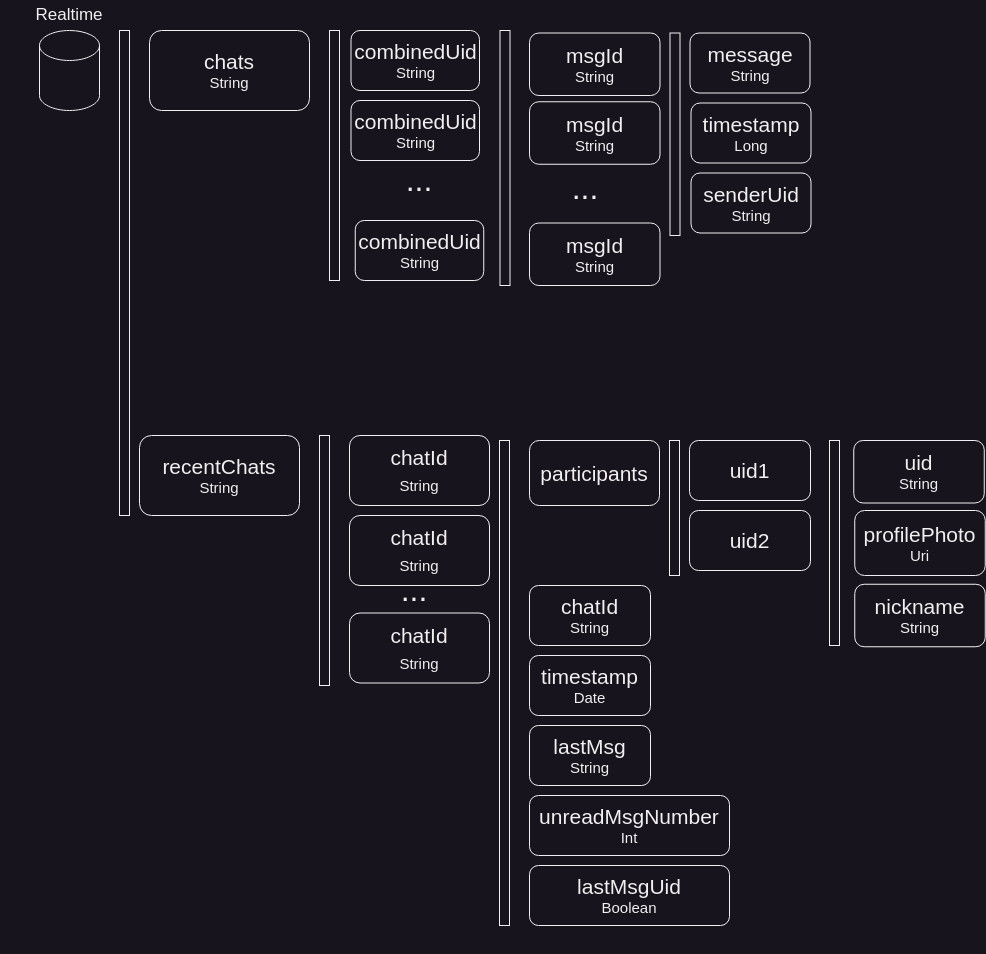
\includegraphics[width = 0.9\textwidth]{Imagenes/drawio/realtime_db.jpg}
	\caption{Diseño de la base de datos Realtime usando Drawio.}
	\label{fig:realtime_db}
\end{figure}

\begin{figure}[ht]
	\centering
	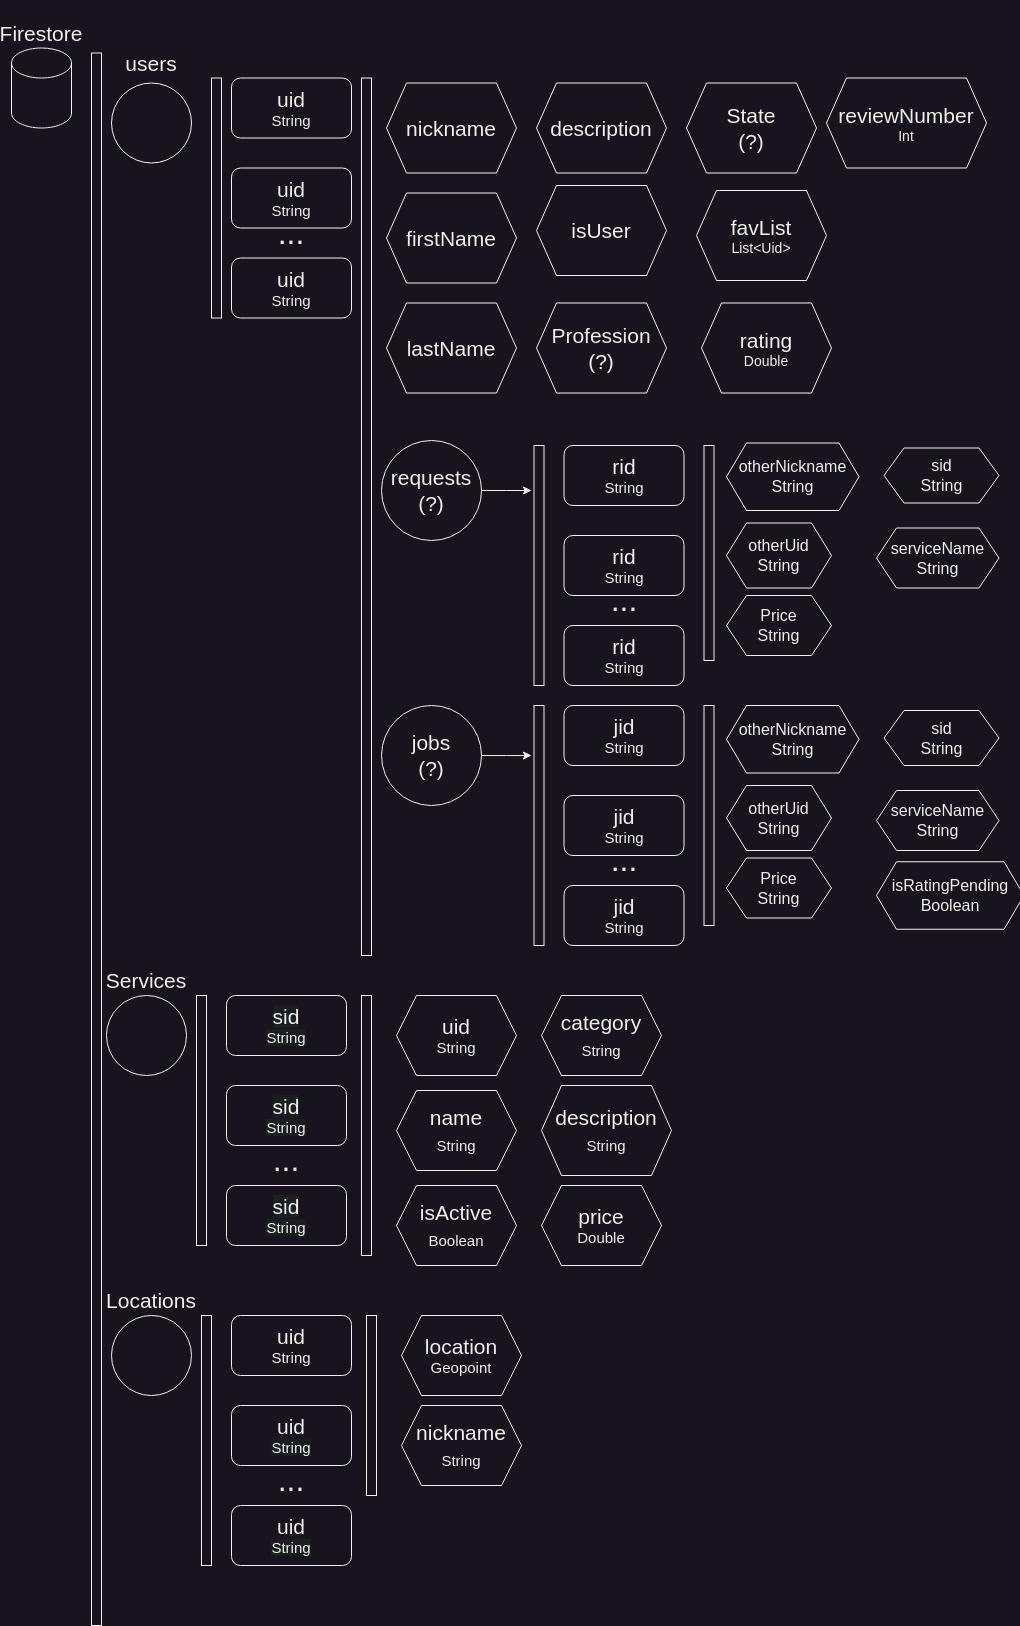
\includegraphics[width = 0.9\textwidth]{Imagenes/drawio/firestore_db.png}
	\caption{Diseño de la base de datos Firestore usando Drawio.}
	\label{fig:firestore_db}
\end{figure}